\documentclass{llncs}

\usepackage{graphicx}
\usepackage[hyphens]{url}
\usepackage{booktabs}
\usepackage{paralist}

% natbib for refs
%\usepackage[numbers,sort]{natbib} 

\begin{document}

\title{``{\emph{Come Together!}}'': Interactions of Language Networks and Multilingual Communities on Twitter}

\author{Nabeel Albishry\inst{1}\thanks{This work has been supported by a doctoral research scholarship for
Nabeel Albishry from King Abdulaziz University, Kingdom of Saudi
Arabia.} \and Theo Tryfonas\inst{1} \and Tom
  Crick\inst{2}}

% \thanks{{\emph{N.B.}} The first part of the title of this paper was
% taken from the motto of the 2016 Eurovision Song Contest, which along
% with the theme artwork was said to be ``inspired by the dandelion,
% symbolising the power of resistance and resilience but also of
% regeneration''.}

\institute{Department of Computer Science, University of Bristol, UK\\\email{\{n.albishry,theo.tryfonas\}@bristol.ac.uk}
\and 
Department of Computing, Cardiff Metropolitan University, Cardiff, UK\\\email{tcrick@cardiffmet.ac.uk}}

\maketitle

\begin{abstract}
Emerging tools and methodologies are providing insight into the
factors that promote the propagation of information in online social
networks following significant activities, such as high-profile
international social or societal events. This paper presents an
extensible approach for analysing how different language communities
engage and interact on the social networking platform Twitter via an
analysis of the Eurovision Song Contest held in Stockholm, Sweden, in
May 2016.  By utilising language information from user profiles
({\emph{N}}=1,226,959) and status updates ({\emph{N}}=7,926,746) to
identify and categorise communities, our approach is able to
categorise these interactions, as well as construct network graphs to
provide further insight on these multilingual communities.  The
results show that multilingualism is positively correlated with
activity whilst negatively correlated with posting in the user's own
language.
 \end{abstract}

\begin{keywords}
Language networks, multilingual communities, community discovery,
network graphs, social networks
\end{keywords}

\section{Introduction}\label{intro}

%\subsection{Online Social Networks}
% 
%In recent years, online social networks have been utilised as
%means to express ideas and opinions, share information about events,
%or even stimulate and propagate calls for civic engagement and
%societal action. Social networking sites such as Twitter, Facebook,
%YouTube and Instagram have also empowered individuals to promote their
%viewpoints and interests -- professional or otherwise -- to a broad
%and diverse global audience. The engagement of certain demographics
%with social networks offers the opportunity for researchers interested
%in observing and interpreting society to apply established theory and
%methods to an emerging digital culture.
%
%To satisfy the demand for various types of communities, interactions
%and engagement, there are now vast numbers of specialist and
%generalist social media sites and platforms, along with a number of
%attempted categorisations. By 2018, there will be an estimated 2.5
%billion active social network users (up from 1.9 billion in 2014);
%they are producing massive amounts of data (volume) on a real-time
%basis (velocity) with implicit sociological attributes such as
%beliefs, opinions, sentiments, behaviours, structures and influences
%(variety)~\cite{burnap-et-al:2015}. These data exhibit the key traits
%of what is referred to as big data: volume, velocity and
%variety~\cite{postsm:2014}. In this age of big social data and an
%increasingly interconnected digital society, there is a new challenge
%-- the application of robust and scalable methods and tools that can
%be applied to digitised social behaviour generated via social networks
%so as to be able to efficiently analyse these big social data to
%provide insight into real-world events and
%actions~\cite{lazer-et-al:2009,burnap-et-al:2015}.
%
%Recent
%work~\cite{blamey-et-al-2012,schwartz-et-al:2013,blamey-et-al-2013,oatley+crick:2014,mostafa-et-al-ai2016}
%has analysed what people say and do on social media to identify
%distinctive words, phrases, and topics as functions of known
%attributes of people such as gender, age, location, or psychological
%characteristics. Data can thus be collated and aggregated, inferring
%gender, age, location and sentiments, from large-scale social media
%data. Potential negative implications of these approaches include the
%fact that they can be easily applied to large numbers of people or
%groups in society without obtaining their explicit consent or even
%being aware it is being done. Data-driven commercial companies,
%governmental entities, or even one's followers or friends are able to
%use software to infer personality and other attributes -- such as
%sexual orientation or political affiliations -- that an individual may
%have decided not to share~\cite{lambiotte+kosinski:2014,postsm:2014}.
%
%There are various projects that have used Twitter corpora and related
%datasets to make predictions about
%elections~\cite{tumasjan-et-al:2010}, stock
%markets~\cite{zhang-et-al:2011}, crimes and
%policing~\cite{gerber:2014,oatley+crick:2015}, even allowing us to
%quantify controversy for topics that spark the most heated debates on
%social media~\cite{garimella-et-al:2016}. Twitter played an important
%role during what was then known as the ``Arab Spring'', which has been
%extensively examined in the social network analysis
%domain~\cite{lotan-et-al:2011,howard-et-al:2011,comunello+anzera:2012,wolfsfeld-et-al:2013,bruns-et-al:2013}.
%While the use of Twitter data has been demonstrated to provide insight
%-- and sociologically relevant demographics~\cite{sloan-et-al:2013} --
%into major social and physical events such as
%riots~\cite{procter-et-al:2013} and terror
%attacks~\cite{burnap-et-al:2014}, often all is not what it may seem;
%for instance, many tweets may not a crowd
%make~\cite{liang-et-al:2013}.

%\subsection{Languages}
% \footnote{\url{https://www.statista.com/statistics/282087/number-of-monthly-active-twitter-users/}}

Despite the widespread use of Twitter globally -- with 328 million
monthly active users as of the first quarter of 2017 -- little
research has investigated the differences amongst users of various
languages; there is a tendency to assume that the behaviours of
English users generalise to other language
users~\cite{hong-et-al:2011}. Language has featured as a facet of
research on the geographies of Twitter
networks~\cite{takhteyev-et-al:2012}, especially whether offline
geography still matters in online social
networks~\cite{kulshrestha-et-al:2012}. Linguistic-inspired studies
have been performed on hashtags~\cite{cunha-et-al:2011}, as well as
the volume and proportional of tweets in English and Arabic, as part
of an analysis of the Arab
Spring~\cite{bruns-et-al:2013}. Nevertheless, language is clearly a
vital component of affiliation and discourse on the
web~\cite{zappavigna+martin:2012}, with the creation and curation of
emerging multilingual networks and communities, representing
well-established creative and cultural norms, including for minority
languages such as Welsh~\cite{gj+uj:2013}, as well as investigations
into the economics of linguistic
diversity~\cite{ginsburgh+weber:2011}.

%\subsection{Social Network Analysis}
In the social network analysis domain, centrality measures such as
degrees, betweenness, clustering coefficient, modularity and cliques
have been used in various projects to measure influence or detect the
emergence of new
communities~\cite{willis-et-al:2015,oatley+crick:2015}.  These
measures provide the ability to assess network graphs that are
constructed from collected data (for example, tweets). Selection of
these centrality measures is dependent on the goal of the analysis;
for example, the degree of a node helps to identify nodes with high
number of connections within the
network~\cite{borgatti+everett:2000,rombach-et-al:2014,liu-et-al:2014}.
In a representation of a real-world network, this metric may help to
identify highly connected persons, such as political leaders, sports
stars or celebrities, who are potential ``information
spreaders''~\cite{cha-et-al:2012,borge-holthoefer-et-al:2012,zhang-et-al:2016}.

Clustering users in communities has been an important factor in social
networking analysis, with a particular focus on clustering users
based on their locations. However, for the sake of anonymity, many
users tend not to disclose information about their identity, such as
locations~\cite{kang-et-al:2013}; looking at Twitter, it has also been
reported in the literature that geotagged tweets are generally low in
number~\cite{morstatter-et-al:2013,tan-et-al:2013,kumar-et-al:2014},
the exponential growth in social media over the past decade has been
joined by the rise of location as a central organising
theme~\cite{liang-et-al:2013} of how users engage with online
information services and, more importantly, with each
other~\cite{cheng-et-al:2010,blamey-et-al-2013,caverlee-et-al:2013}. The work here
examines the correlation between multilingualism of users and their
associated activity.

%\subsection{Overview of Paper}

The remainder of this paper is organised as follows: in
Section~\ref{methodology}, we introduce the methodology and key
language themes; Section~\ref{results} presents the 2016 Eurovision
Song Context case study, along with an analysis of the key data and
results; Section~\ref{conclusions} concludes the paper with a wider
discussion and a summary of the potential application of our approach.


\section{Methodology}\label{methodology}

The primary purpose of this study is to identify and define an
extensible analytical approach for examining language uses,
communities, and diversity on Twitter. The approach is based on
network graphs and their properties, such as indegree, outdegree, and
edge weights. Graphs are generated from language settings in users'
profiles and those for statuses.  First, we construct user graphs to
analyse interactions and multilingualism at the level of individual
users. Then, from the user graphs, we produce language communities
graph that groups users based on common languages.

\section{Language Entities}

To generate the required graphs, we need three essential entities from
each status; user ID, user profile language, and status
language\footnote{For Twitter, \emph{status} may also be referred to
as \emph{post}, or \emph{tweet}.}.  Those values can be extracted from
{\emph{[status][`user'][`id']}}, {\emph{[status][`user'][`lang']}},
and {\emph{[status][`lang']}}, respectively. It is important to note
that the focus of this work is on the analytical approach, not
necessarily the accuracy of language detection; therefore we assume
that language of tweets are correctly identified via the user profile.
For profiles, users are expected to pick a language for their
settings. Nevertheless, their language entity may show as the initial
placeholder text ``\emph{Select Language...}'' or a translated version
that may provide information to the user's native language community.

% \subsection{Users and Locations}
% It is important to understand how geotagging works in Twitter. The
% `{\emph{place}}' entity included in a Twitter status does not
% necessarily indicate precisely where the actual posting was made, as
% stated in the Twitter API
% documentation\footnote{\url{https://dev.twitter.com/overview/api/places}}:
% ``{\emph{Tweets associated with places are not necessarily issued from
% that location but could also potentially be about that
% location}}''. For the sake of anonymity, many users tend not to
% disclose information about their identity, particularly locations;
% this has also been supported by the literature that geotagged tweets
% are generally low in number~\cite{kang-et-al:2013}. We took the step
% to verify this claim in our datasets; in the best cases, the ratio of
% geotagged tweets did not exceed 2\%.

% In the case of the
% {\texttt{\#BaltimoreRiots}} dataset, only ~1\% of collected statuses
% were associated with places. Moreover, out of this geotagged subset,
% only 4\% were associated with the city where the event took place
% (Baltimore).

% An alternative location-based option to consider is based on profile
% location, but it still does not serve the need for location clustering
% for a multitude of reasons. Firstly, we found that less than 45\% of
% users have set their profile location, which is in line with other
% studies~\cite{graham-et-al:2014}. Secondly, although Twitter suggests
% certain presets for setting profile location, users are given the
% option to enter any text they wish; this results in a considerable
% amount of noise.

\subsection{Network Graphs}\label{netgraphs}

For this study, we need to generate two different graphs; one is based
on individual users and their posting activity, while the other
combines users into language communities. In the context of this
study, all graphs must be directed to provide correct measurements, as
demonstrated in Figure~\ref{fig:graphstructures}.

\begin{figure}[htb]
\centering
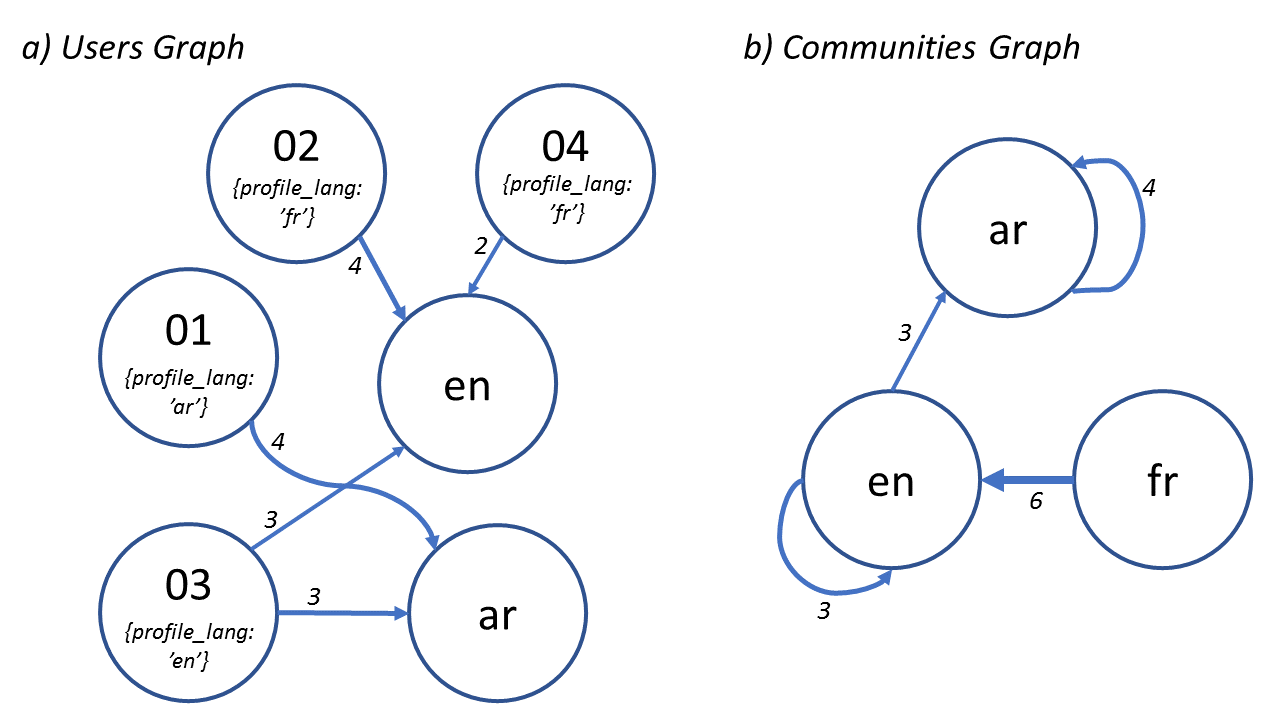
\includegraphics[width=0.9\columnwidth]{images/graphstructures.png}
\caption{Examples of simple models of language graphs}
\label{fig:graphstructures}
\vspace{-2em}
\end{figure}

\subsubsection{User Graph}

This graph represents the core structure for our analysis. As shown in
Figure~\ref{fig:graphstructures}(a), nodes in this graph are of two
types; users and posting language. Each posted tweet resulted in two
nodes, one represents the user with profile language setting added to
the node as the attribute `{\emph{\{profile\_lang:xx\}}}'. The other
node represents language of the tweet. Edges link users with the
posting languages they used, and their weight (thickness) measures the
number of tweets that have been posted by the user (the starting node)
in the target language (ending node).  In the example above, the
profile language setting for user `{\emph{03}}' is `{\emph{en}}', they
posted three tweets in `{\emph{en}}' and three in `{\emph{ar}}'
(Arabic). This graph will be referred to as the \emph{user graph}.

\subsubsection{Communities Graph}\label{communitiesgraph}

This second graph is derived from the user graph and has one type of
node to represent language community, as shown in
Figure~\ref{fig:graphstructures}(b).  For each user node we generate
one node from the `{\emph{\{profile\_lang:xx\}}}' attribute, and
another node from the posting language to which it is connected. This
resulted in combining all users of the same profile language into one
node, with edge connecting to posting language and its weight
measuring their activity. Theoretically, each tweet results in two
language nodes, one for the user profile, and the other for language
of the tweet. In our example above, users with `{\emph{fr}}' (French)
profiles have generated six tweets in `{\emph{en}}'. In the case of
`{\emph{ar}}' node, we can see that users of the profile language as
`{\emph{ar}}' have posted four tweets in `{\emph{ar}}' only -- in
graph terminology this is referred to as `self-loop'; we will refer to
this graph as the {\emph{communities graph}}.

Throughout the paper, we refer to language communities in two ways;
{\emph{profile community}} to perceive the language as user profile
settings, whereas {\emph{posting community}} refers to the language as
tweeting settings.

\subsection{Measures}

In this section, we will discuss how graph measures can be used to
make deductions about users, associated community languages, posting
language activity, and how different language communities are linked
to each other.  These measures and their interpretations, in the
context of this study are as follows:\\

\begin{compactitem}
\item \emph{Indegree}: number of incoming edges;
\item \emph{Outdegree}: number of outgoing edges;
\item \emph{Edge Weight}: number of tweets on edge;
\item \emph{Weighted indegree}: total weights of incoming edges;
\item \emph{Weighted outdegree}: total weights of outgoing edges.
\end{compactitem}

\subsubsection{User Graph Properties}

User nodes have {\emph{indegree}}=0, and posting languages have
{\emph{outdegree}}=0; these two properties will be used to distinguish
between nodes. Both outdegree of user nodes and indegree of posting
languages must be greater than 0. The edge weight indicates the number
of tweets associated with both end nodes. Referring to the example in
Figure~\ref{fig:graphstructures}(a), we can see that user
`{\emph{03}}' has indegree of 0 (user identifier), outdegree of 2
(number of languages he used), and weighted outdegree of 6 (total
number of tweets posted). Also, in the same figure, we can see that
for `{\emph{en}}' posting language, it has outdegree of 0 (language
nodes identifier), indegree of 3 (number of users posted in this
language), and weighted indegree of 9 (total number of tweets posted);
Table~\ref{tbl:usersgraph} presents main properties of this graph.

\begin{table}[htb]
\centering
\caption{Node properties in user graph}
\begin{tabular}{@{}lrr@{}}
\toprule
\textbf{}& \textbf{User} & \textbf{Language} \\ \midrule
{\emph{Indegree}} & 0 & \textgreater0 \\
{\emph{Outdegree}} & \textgreater0 & 0 \\ 
{\emph{Edge Weight}}& \multicolumn{2}{c}{\#Tweets}\\ \bottomrule
\end{tabular}
\label{tbl:usersgraph}
\vspace{-2em}
\end{table}

\subsubsection{Communities Graph Properties}

As discussed in Section~\ref{communitiesgraph}, this graph is
extracted from the user graph and contains one type of node: language
community nodes. Nodes in this graph represent languages as profile
language settings, posting language, or both.  However, as the graph
is directed, we can identify if a community node is for profile or
posts by measuring the \emph{indegree} and \emph{outdegree}
properties.  Positive indegree implies posting language, and positive
outdegree indicates profile language settings. Figure
\ref{fig:graphstructures}(b) shows three language communities, two
nodes appear as posting and profile nodes, while one node exists as a
profile only node. The node `{\emph{ar}}', for example, has outdegree
of 1 and indegree of 2.  In other words, at least one user has their
profile language settings as `{\emph{ar}}', and at least two users
have posted in `{\emph{ar}}'. In terms of edge weights, we can say
that there are seven tweets posted in `{\emph{ar}}' language,
originated from two different profile language communities.  For the
`{\emph{fr}}' node, we can see only outdegree, which means this
language community exists as a profile-only node as no user posted in
`{\emph{fr}}'; these measures are summarised in Table
\ref{tbl:communitiesgraph}.

\begin{table}[htb]
\centering
\caption{Node properties in communities graph}
\begin{tabular}{@{}lrr@{}}
\toprule
\textbf{}& \textbf{Community Node} \\ \midrule
{\emph{Indegree}} &  posts\\
{\emph{Outdegree}} & profiles \\ 
{\emph{Edge Weight}}& \#Tweets\\ \bottomrule
\end{tabular}
\label{tbl:communitiesgraph}
\end{table}

% We present two language diversity measurements. The
% first, which we call `diversity', is to measure uses of languages
% different to the profile's i.e. we are referring to `non-selfloop'
% edges in the generated network graphs. The second one is to measure
% the magnitude of this diversity, which can be calculated as the total
% weight of `non-selfloop' over total edge weights in the
% profile-posting graph. We will make observation on these two
% measurements for both cases.

% By observing the language diversity of profile communities, we aim to
% measure language diversity of the topic in general. The same technique
% can be applied on individual communities within the topic. By doing
% so, it can help identify communities that act as bridges between
% different profile communities. Moreover, the technique can be applied
% to measure diversity at individual users level.

% \section{Case Study: 2015 Baltimore Protests}\label{baltimorecasestudy}

% Following a peaceful funeral that took place on the morning of Monday
% 27 April 2015 in Baltimore, Maryland, USA, a protest hit the
% city. According to the timeline published on the CNN website
% ``{\emph{The city exploded on Monday after the funeral of Freddie
% Gray, a 25-year-old black man who mysteriously died on April 19, a
% week after Baltimore Police arrested
% him.}}''~\cite{baltimorewiki:2015}. The nature of the Baltimore
% protests is a good representation of a partially planned event in
% which a sudden escalation of civil unrest hits a geographical area. The
% event manifested itself on Twitter as {\texttt{\#BaltimoreRiots}}, and
% resulted in more than 1,250,000 status updates.

% Figure~\ref{fig:overallbaltimoreactivity} shows how the event
% manifested itself on Twitter once a ``purge'' was scheduled. We can
% see that what was happening on the ground was quickly reflected in the
% online activity on Twitter. More detailed analysis reveals that within
% one hour the topic started to go ``viral''; more precisely, at
% approximately 15:00 on 27 April at which the ``purge'' was
% scheduled. The topic jumped from roughly 1,200 to 8,000 tweets per
% hour. Then, it peaked with 98,000 between 22:00 and 23:00.

% \begin{figure}[htb]
% \centering
% 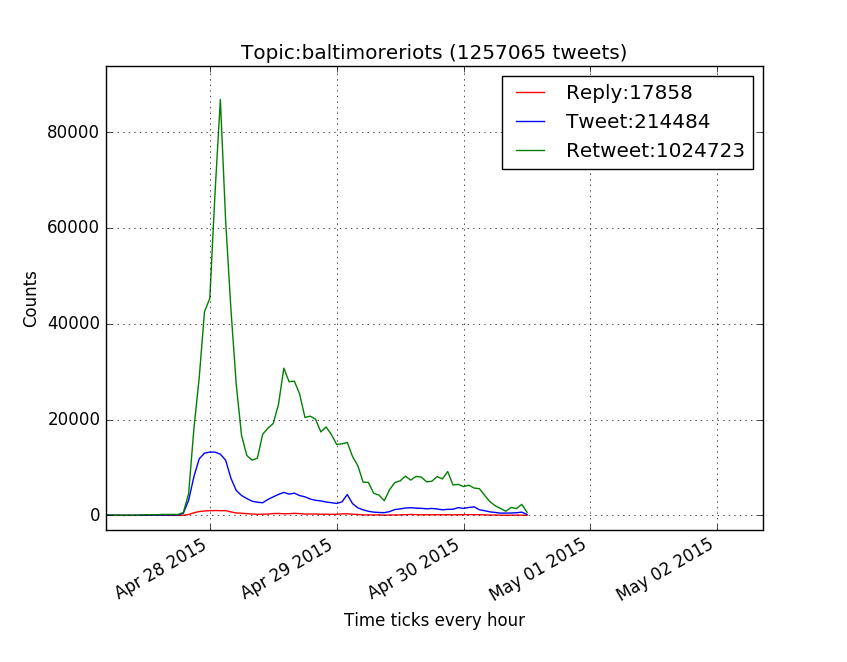
\includegraphics[width=\columnwidth]{images/overallbaltimoreactivity.png}
% \caption{Overall activity for {\texttt{\#BaltimoreRiots}}.}
% \label{fig:overallbaltimoreactivity}
% \end{figure}

% \subsection{Posting Communities}\label{baltimoreposting}

% In the {\texttt{\#BaltimoreRiots}} case, 38 posting languages were
% used for original posts. As we can see in
% Figure~\ref{fig:baltimore_langfreq}, English was the mostly
% frequently-used language by far. Interestingly, results also show that
% language of more than c.7\% statuses could not be identified. When
% investigated, those statuses mostly did not contain text other than
% hashtags, pictures or URLs. Although, this is not a big proportion of
% the overall sample, it came second after English. This category shows
% an interesting case in which qualitative content analysis could
% potentially be used, but it is beyond the scope of this study and will
% not be covered here.

% \begin{figure}[htb]
% \centering
% 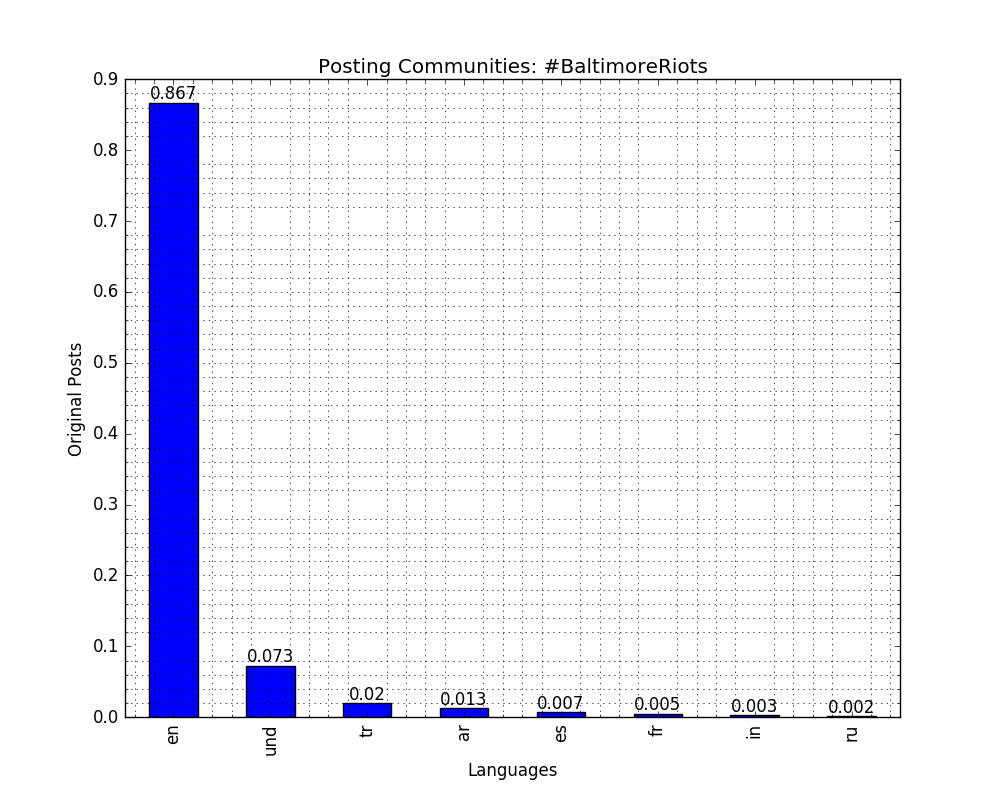
\includegraphics[width=\columnwidth]{images/baltimore_langfreq.png}
% \caption{Most frequently used languages in
%   {\texttt{\#BaltimoreRiots}}: 
% ({\emph{en:}} English; {\emph{es:}} Spanish; {\emph{tr:}} Turkish;
%   {\emph{fr:}} French; {\emph{en-gb:}} British English; {\emph{ar:}}
%   Arabic; {\emph{de:}} German; {\emph{ru:}} Russian; {\emph{it:}}
%   Italian; {\emph{pt:}} Portuguese)}
% \label{fig:baltimore_langfreq}
% \end{figure}

% \subsection{Profile Communities}\label{baltimoreprofile}

% In the majority of cases, users choose to pick a language for their
% Twitter profile settings. In our dataset, we found that out of 716,494
% users, only 45 had not opted to select a language. However, the
% language entity returned by the API for those cases is the initial
% placeholder text ``{\emph{Select Language...}}'' or a translated
% version that may provide hints to the user language
% community. Figure~\ref{fig:baltimore_profile_size} shows that about
% 94\% of the users came from `{\emph{en}}' profile community.

% \begin{figure}[htb]
% \centering
% 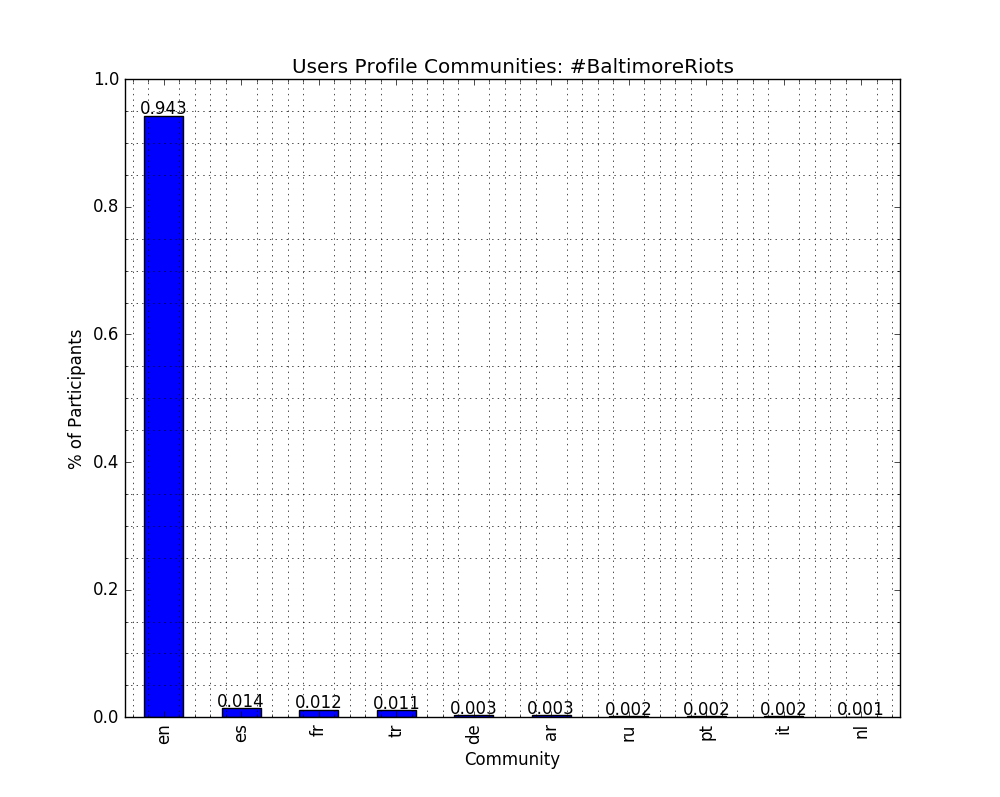
\includegraphics[width=\columnwidth]{images/baltimore_profile_size.png}
% \caption{Top 10 profile language communities in {\texttt{\#BaltimoreRiots}}}
% \label{fig:baltimore_profile_size}
% \end{figure}

% \begin{figure}[htb]
% \centering
% 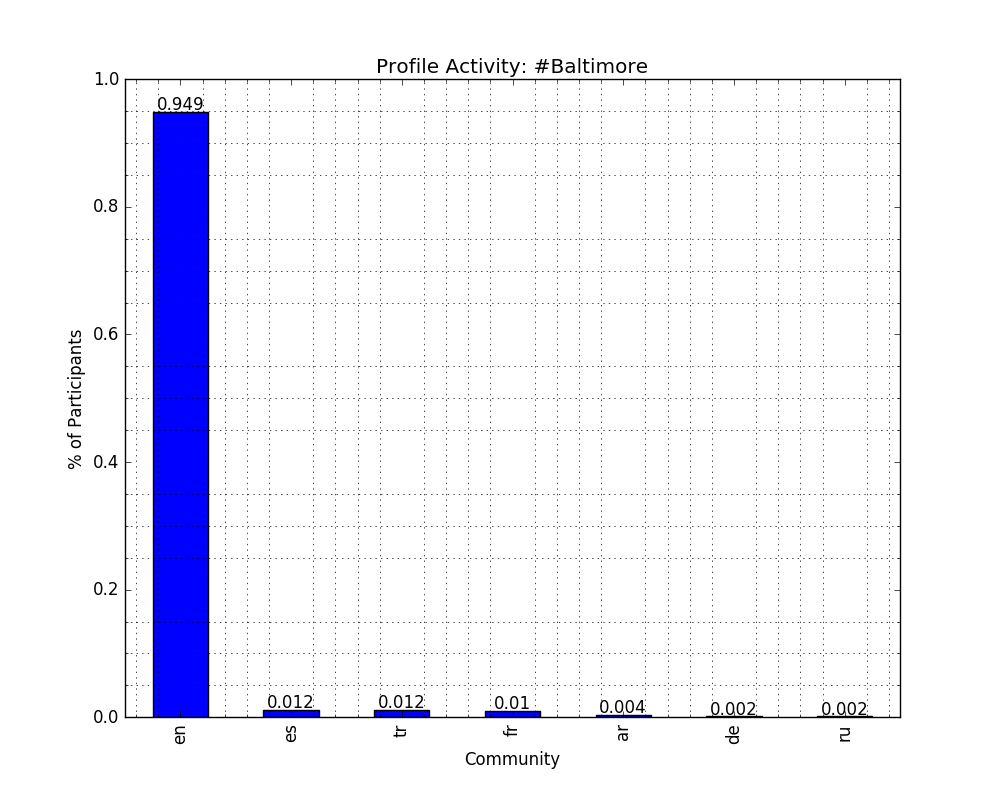
\includegraphics[width=\columnwidth]{images/baltimore_profile_activity.png}
% \caption{Profile language communities causing \%99 of activity in {\texttt{\#BaltimoreRiots}}}
% \label{fig:baltimore_profile_activity}
% \end{figure}

% As we can see in Figure~\ref{fig:baltimore_profile_activity}, activity
% from profile communities is not far from their relative sizes.  Also,
% from these two outputs, we can see that nearly all of the topic
% activity came from one particular community using one particular
% language. This extreme pattern may accompany extreme and
% geographically constrained real-world events such as civil unrest and
% terrorist attacks.

% \subsection{Profile-Posting Network}

% This section explores the network graph we are able to build from
% profile-posting relationships; constructing this graph is an essential
% step for our core analysis of language diversity. For example, to
% investigate whether the `{\emph{en}}' posting community is linked to
% particular profile communities, we used the bipartite graph as
% presented in figure~\ref{fig:baltimore_p_s_lang_sl}.  In this graph,
% nodes that are prefixed by ``{\emph{p\_}}'' represent profile language
% community, and nodes that are prefixed by ``{\emph{s\_}}'' represent
% posting language community. The size of node represents the weighted
% indegree, whereas colour represents the outdegree: the darker the
% colour, the higher outdegree; hence, completely white nodes have no
% outdegree and help to easily distinguish posting communities from
% profile ones. From the graph we can infer that there is a dominating
% player in both domains: posting languages and profile communities.
% Therefore, for the case of {\texttt{\#BaltimoreRiots}}, we can
% conclude that the case was substantially localised.

% \begin{figure*}[!htb]
% \centering
% 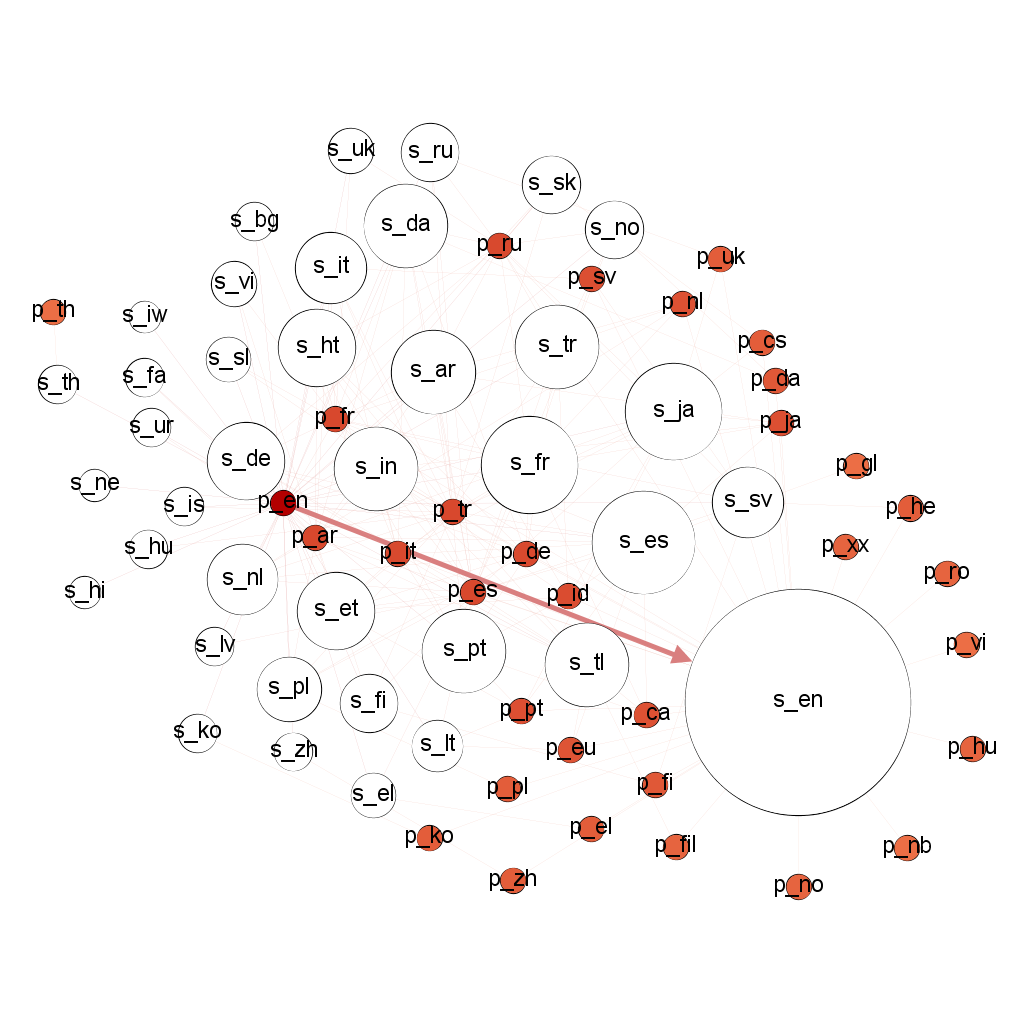
\includegraphics[width=0.8\textwidth]{images/baltimore_p_s_lang_sl.png}
% \caption{Profile-posting network graph}
% \label{fig:baltimore_p_s_lang_sl}
% \end{figure*}


% \subsection{Diversity and Multilingual Communities}

% To examine users' behaviour in using languages other than their own
% (profile language), same-language communities are filtered out.  We
% found that English profile users frequently posted in Arabic, as a
% secondary posting language. This sort of activity could be obtained
% from edge weights in the profile-posting
% graph. Table~\ref{tbl:baltimoredifflang} shows the top portion of
% these communities. This observation sheds light on those
% relationships, and could be of use for further analysis, such as
% identifying highly disseminated message that fall into these
% relationships and their contents.

% \begin{table}[!htb]
% \centering
% \caption{Users' behaviour in using languages different to their profile (normalised)}
% \begin{tabular}{@{}lcr@{}}
% \toprule
% \textbf{Profile-Posting Edge} & \textbf{Weight} \\ \midrule
% {\emph{en-ar}} & 1.00 \\
% {\emph{es-en}} & 0.49 \\
% {\emph{ar-en}} & 0.47\\ 
% {\emph{fr-en}} & 0.38 \\
% {\emph{tr-en}} & 0.37 \\
% {\emph{en-tr}} & 0.36 \\ \bottomrule
% \end{tabular}
% \label{tbl:baltimoredifflang}
% \end{table}

% The topic diversity in {\texttt{\#BaltimoreRiots}} is 0.91, which is
% not surprising when we recall that there were 38 languages used in
% original tweets. However, when the magnitude of diversity was
% measured, it gave a score of 0.04, a generally low score. This will be
% of use when compared to the data from our second case study in Section
% ~\ref{eurovisioncasestudy}.

% Additionally, measuring multilingual communities is another use of
% profile-posting network graph at individual users' level. We grouped
% users based on their relationship with posting communities, regardless
% of their profile language. For example, a user posting in both
% `{\emph{en}}' and `{\emph{fr}}' will be classified as bilingual, and
% so on. Based on this grouping technique, with the `{\emph{und}}' lang
% category eliminated, we identified nine sets. As we can see in
% Figure~\ref{fig:baltimore_multilingual}, monolingual group contain the
% overwhelming majority of users (nearly 99\%), contributing
% approximately 94\% of the topic activity too.

% \begin{figure}
% \centering
% 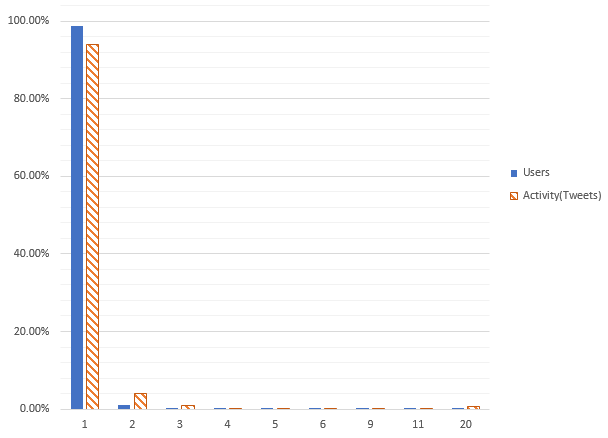
\includegraphics[width=\columnwidth]{images/baltimore_multilingual.png}
% \caption{Multilingual communities and their activity in {\texttt{\#BaltimoreRiots}}}
% \label{fig:baltimore_multilingual}
% \end{figure}

% FUDGE
\vspace{-3em}

\section{Case Study and Discussion}\label{results}

% The Eurovision Song Contest is the longest-running annual
% international TV song competition, held, primarily, among the member
% countries of the European Broadcasting Union since 1956. Each
% participating country submits an original song to be performed on live
% television and radio and then casts votes for the other countries'
% songs to determine the most popular song in the competition. The
% contest has been broadcast every year for sixty years, and is one of
% the longest-running television programmes in the world. It is also one
% of the most watched non-sporting events in the world, with audience
% figures varying in recent years from 100 million to 600 million
% globally\footnote{\url{https://www.eurovision.tv}}. The emergence of
% social networking in recent years has dramatically changed the range
% and scope of audience interaction and engagement, particularly for
% different language communities.

In our case study, we explore the analysis of a dataset collected from
the {\texttt{\#Eurovision}} hashtag during the 2016 Eurovision Song
Contest, based on the techniques presented in
Section~\ref{methodology}. Using the \emph{user graph} and
\emph{communities graph}, we conduct analyses on multilingualism,
activities and user behaviours in posting in different
languages\footnote{In this context, \emph{different language} refers
to tweet's language that is different to the user profile language
settings.}.

\subsection{Case Study: 2016 Eurovision Song Contest}\label{context}

The 2016 Eurovision Song
Contest\footnote{\url{https://www.eurovision.tv/page/stockholm-2016/all-participants}}
took place in May in Stockholm, Sweden, with the motto of
``{\emph{Come Together!}}''. There were 32 countries taking part, with
two semi-finals taking place on 12 and 14 May, with 26 countries
qualifying for the final on 16 May. This year's contest was perceived
by many commentators to be tense and politically motivated, especially
with Ukraine eventually winning the
final~\cite{telegrapheuroboycott:2016}. Varying analyses see the
contest as being influenced by political conflicts, friendships or
cultural
bias~\cite{ginsburgh+noury:2008,charron:2013,blangiardo+baio:2014,budzinski+pannicke:2016},
with a range of news articles explicitly discussing the possibly
biased results~\cite{telegrapheurobias:2016}.  Twitter activity was
very high throughout the event on the primary {\texttt{\#Eurovision}}
hashtag, with close to 8 million statuses, produced by nearly 1.25
million users.

% \begin{figure}[htb]
% \centering
% 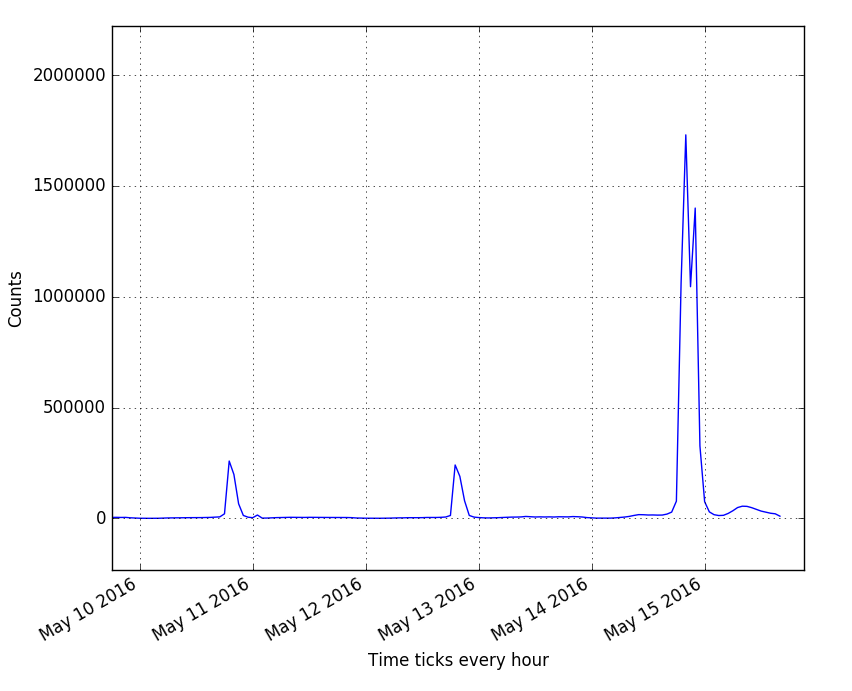
\includegraphics[width=0.6\columnwidth]{images/overalleurovisionactivity.png}
% \caption{Overall activity for {\texttt{\#Eurovision}}.}
% \label{fig:overalleurovisionactivity}
% \end{figure}

The study focuses on original statuses (tweets) as the basic entity,
as we wish to measure posting behaviour, not reactions. Preliminary
analysis shows that they account for 48\% of the total activity, of
which 4\% tweets with an `{\emph{unidentified}}' language were
eliminated. As for profiles, all users have chosen language
preferences and no profile was found with the default language
settings.


\subsection{Multilingualism}

The outdegree in the user graph shows the number of languages a user
used; observing the outdegree of user nodes in the users graph revealed 20
groups of outdegree, ranging from 1 to
25. Figure~\ref{fig:multilingual} shows these groups, size of users
and activities. Although 85\% of users are monolingual, their
activity accounts for 47\% of all tweets. Additionally, while the
average activity of users is five posts per user, monolingual users
were the least active ones, scoring an average of two tweets per
user. We found that 18\% of tweets were in different languages, with a
strong correlation between multilingualism and likelihood of using
different languages.

\begin{figure}[htb]
\centering
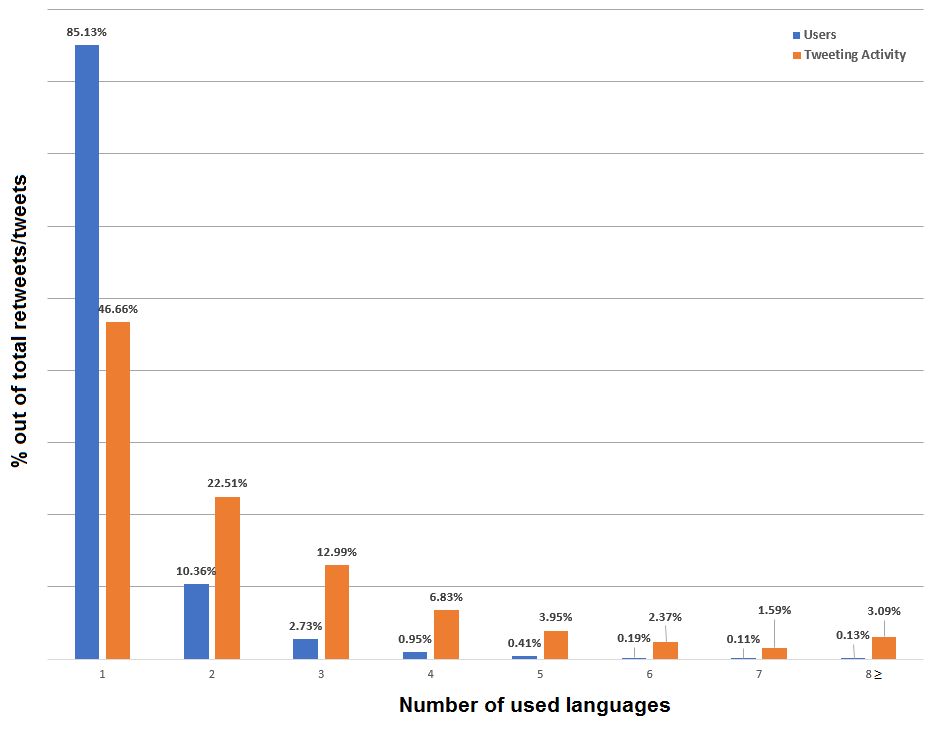
\includegraphics[width=0.9\columnwidth]{images/multilingualcommunities.png}
\caption{Multilingual communities on {\texttt{\#Eurovision}} and their associated activities.}
\label{fig:multilingual}
\end{figure}

We used the user graph to generate two communities graphs; the first
will be used to explore language communities amongst monolingual
users, while the other includes language communities for multilingual
users only.

%In these graphs we chose to 
%focus on active users only, therefore we eliminated users with activity lower than the overall 
%average, i.e. 5 tweets per user.

\subsection{Monolingual Communities}

This graph includes 63 language communities: 15 languages exist as
profile-only and have not been used in any post, while 12 were used in
posting but never show as a profile language. Moreover, about 13\% of
monolingual users used different languages in posts which form 10\% of
tweets in monolingual communities. Hence, strongest relationships
exist as a self-loop, as discussed in
Section~\ref{communitiesgraph}.

To explore the relationships between language communities, we remove
all self-loop edges from the graph. The resultant graph shows that
monolingual users with `{\emph{en}}' as profile language have posted
in 47 other languages, causing 43\% of tweeting activity, and that 48
other profile communities used `{\emph{en}}' language in posting
43\%. Also, we found that the strongest relationship (edge weight),
9\% of activity, is when `{\emph{en}}' profiles post in `{\emph{es}}'
(Spanish). A further interesting case to mention involve the `\emph{el}'
(Greek) and `\emph{ru}' (Russian) languages. Although the number of
profile communities that used `\emph{ru}' is more than twice compared to
the number of those that used `\emph{el}', they were significantly lower
in terms of activity.

%\begin{table}[htb]
%\centering
%\caption{Nodes properties in communities graph}
%\begin{tabular}{@{}lcr@{}}
%\toprule
%\textbf{Language} & \textbf{Indeg} & \textbf{Outdeg} \\%& \textbf{Posting} & \textbf{Profile} \\ 
%\midrule
%{\emph{en}} & 35 & 32 \\
%{\emph{es}} & 13 & 6  \\ 
%{\emph{de}} & 10 & 2\\ 
%{\emph{es}} & 13 &  2\\ 
%{\emph{de}} & 10 & 10 \\ 
%\bottomrule
%\end{tabular}
%\label{tbl:communitiesgraph}
%\end{table}

% \begin{table}[!htb]
% \centering
% \caption{Users' behaviour in using languages different to their profile (normalised)}
% \begin{tabular}{@{}lcr@{}}
% \toprule
% \textbf{Profile-Posting Edge} & \textbf{Weight} \\ \midrule
% {\emph{en-ar}} & 1.00 \\
% {\emph{es-en}} & 0.49 \\
% {\emph{ar-en}} & 0.47\\ 
% {\emph{fr-en}} & 0.38 \\
% {\emph{tr-en}} & 0.37 \\
% {\emph{en-tr}} & 0.36 \\ \bottomrule
% \end{tabular}
% \label{tbl:baltimoredifflang}
% \end{table}

\subsection{Multilingual Communities}

Although multilingual users form 15\% of all users in the dataset,
they generated 53\% of tweeting activity. There are 48 language
communities in this graph, 13 languages as profile-only, and 10 as
posting languages. With self-loop edges excluded, activity in
different languages measured 24\% of multilingual users tweets. Also,
we found that the strongest relations existed between the `\emph{es}'
profile community and the `\emph{en}' posting language, which is the
opposite to the monolingual case.
%The following table shows top multilingual 
%communities, ordered by their \emph{weighted indegree}.


\subsection{Visualisation}

In Figure~\ref{fig:communitiesgraphs}, we present two communities
graphs; the size of the node represents weighted indegree of
community; how much a language was used in tweeting, and darkness
reflects weighted outdegree; participation from users of language
community. Edges link between \emph{profile} and \emph{posting}
communities, and their thickness indicates the number of tweets
posted.

\begin{figure}[htb]
\centering
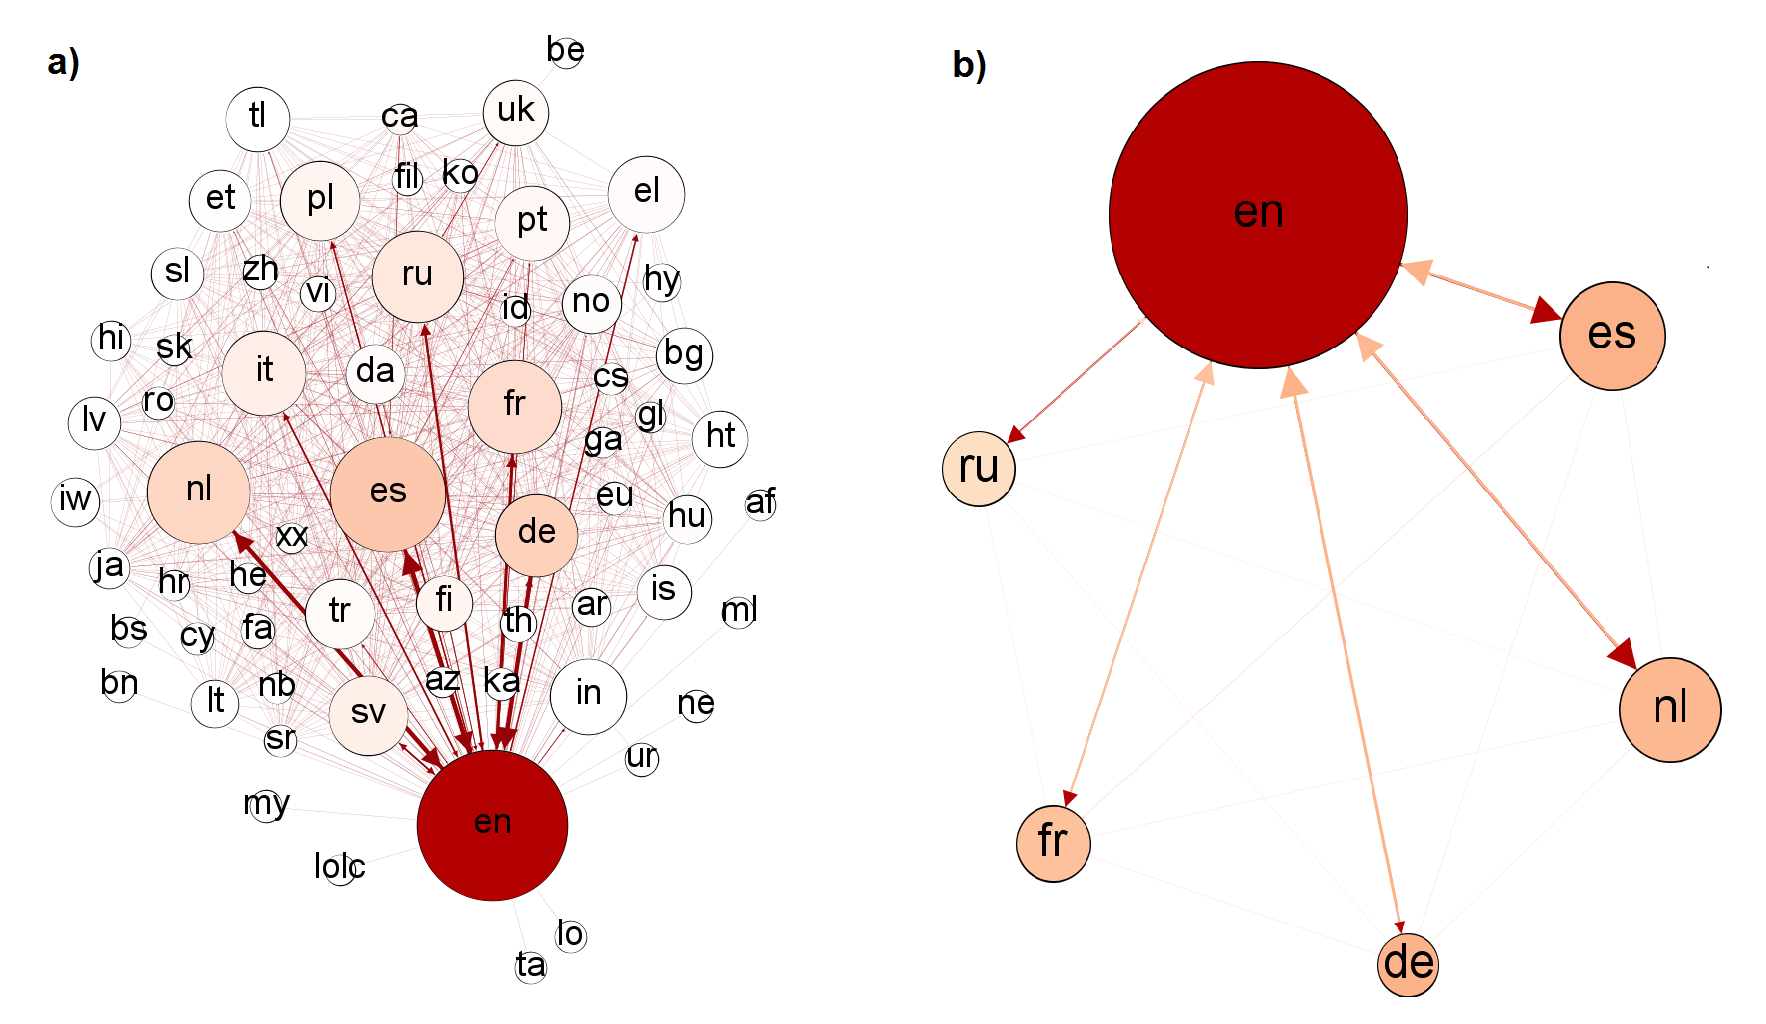
\includegraphics[width=0.9\textwidth]{images/communitiesgraphs.png}
\caption{Language Communities Graphs for {\texttt{\#Eurovision}}.}
\label{fig:communitiesgraphs}
\end{figure}

Whilst Figure~\ref{fig:communitiesgraphs}(a) shows all language
communities together, \ref{fig:communitiesgraphs}(b) presents a
filtered graph. This filtered graph depicts relationships amongst
language communities that scored high in weighted indegree and
outdegree. Also, we eliminated users with activity lower than the
overall average (five tweets/user), and generated the communities
graph from the remainder.


%\begin{figure}[htb]
%\centering
%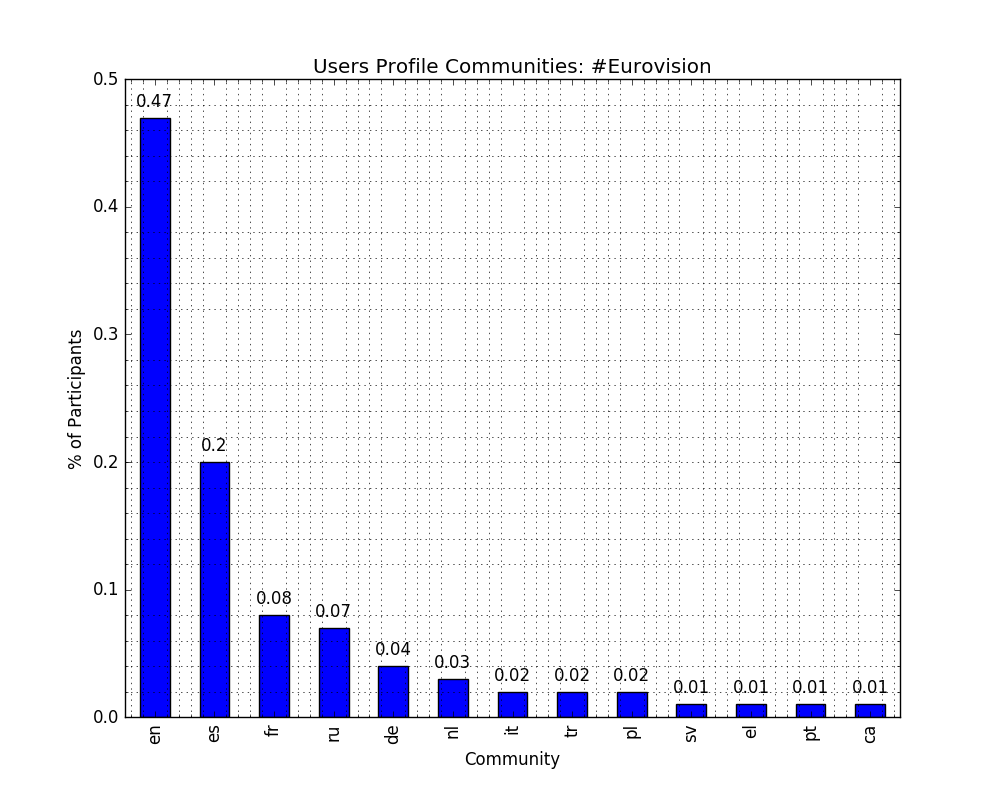
\includegraphics[width=\columnwidth]{images/eurovision_profile_size.png}
%\caption{Profile communities by size in {\texttt{\#Eurovision}}.}
%\label{fig:eurovisionprofilesize}
%\end{figure}

%\begin{figure}[htb]
%\centering
%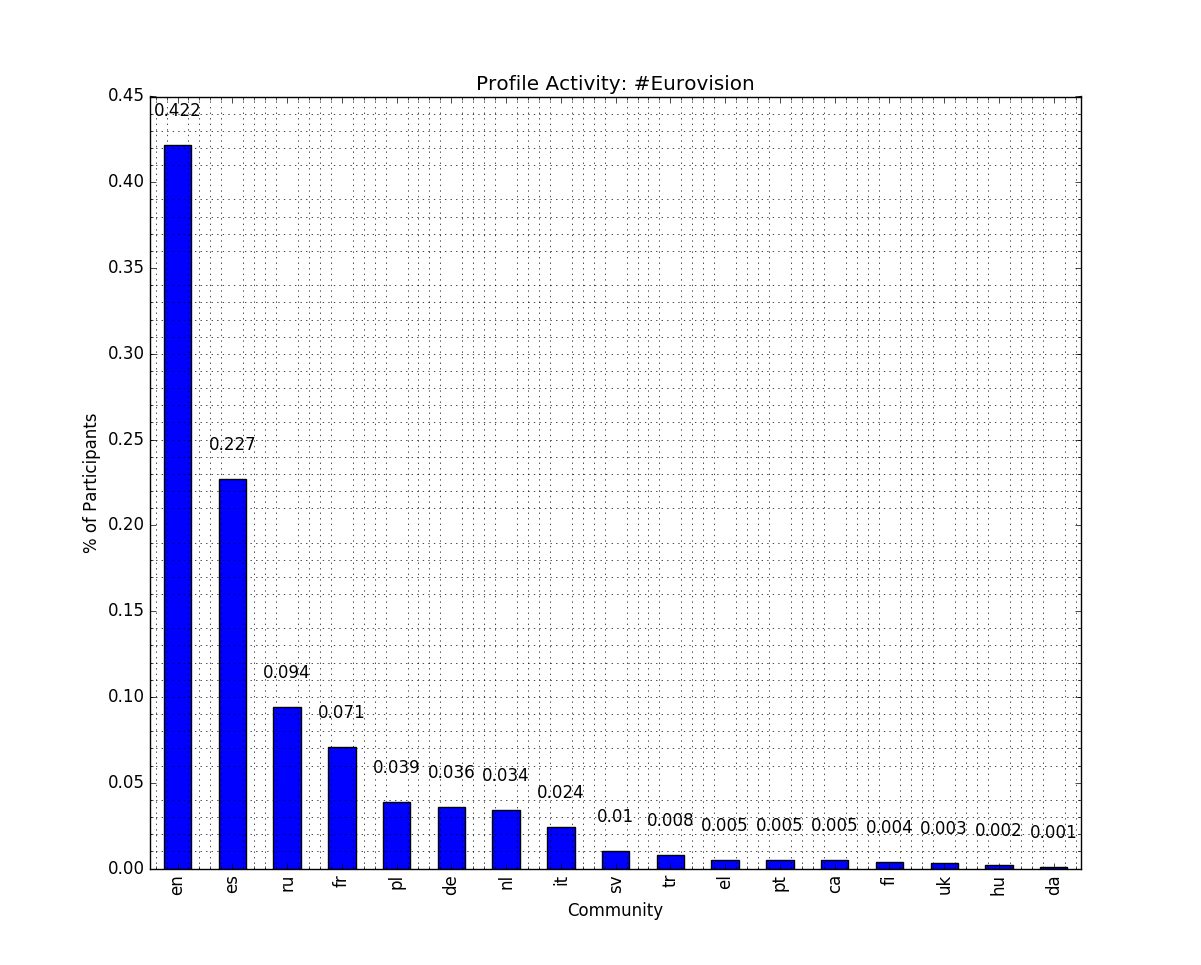
\includegraphics[width=\columnwidth]{images/eurovision_profile_activity.png}
%\caption{Profile communities by activity in {\texttt{\#Eurovision}}.}
%\label{fig:eurovisionprofileactivity}
%\end{figure}

% \begin{figure*}[!htb]
% \centering
% 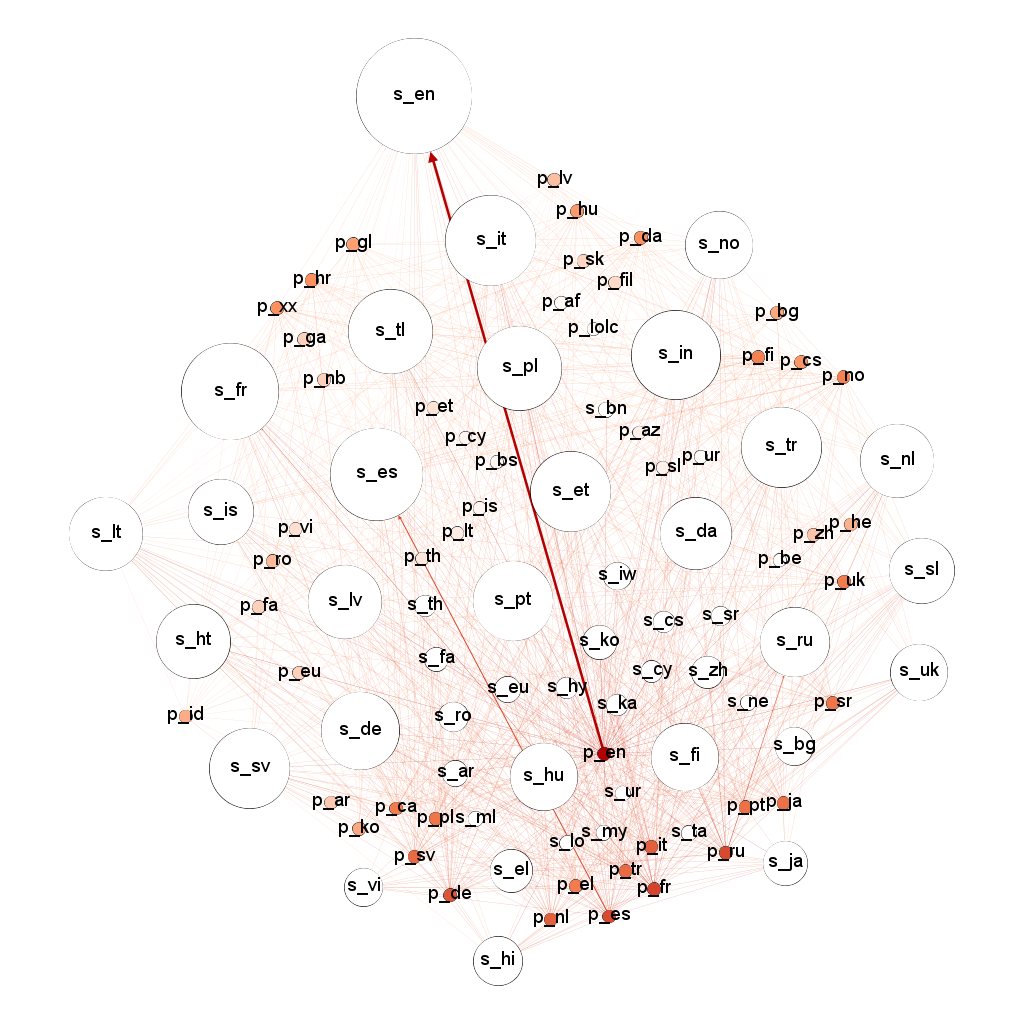
\includegraphics[width=0.8\textwidth]{images/euro_pslang.png}
% \caption{Profile-posting network graph for {\texttt{\#Eurovision}}}
% \label{fig:eurovisionpslang}
% \end{figure*}

% \subsection{Profile-Posting Analysis}\label{eurovisionppanalysis}

% To explore the posting behaviour from profile communities, we
% constructed the graph shown in Figure~\ref{fig:eurovisionpslang},
% allowing us to continue analysing the '{\emph{fr}}' and '{\emph{ru}}'
% example.  The graph helps us to evaluate contributions of profile
% communities to the Russian posting community, with Russian language
% profile communities resulted in more than 95\% of activity in this
% posting community. The relative weights from those profile communities
%to the Russian posting community were {\emph{ru}}: 91.25\% and
%{\emph{en}}: 7.26\%.

% \begin{table}[!htb]
% \centering
% \caption{Active profile communities within the Russian posting community}
% \begin{tabular}{@{}lc}
% \toprule
% \textbf{Community} & \textbf{\%} \\ 
% \midrule
% {\emph{ru}} & 91.25 \\
% {\emph{en}} & 7.26 \\
% \bottomrule
% \end{tabular}
% \label{tbl:russian}
% \end{table}

% However, posts in Russian were not just appearing from the Russian profile
% community. This show one way of exploring relationships between
% profile and posting communities, especially if we are interested in
% particular communities. Another approach is to explore the posting
% behaviour of one particular community. When considering certain
% profile communities, there is a tendency to assume that communities
% only post in languages that are the same as their profile language. To
% examine this assumption, we investigated participation of
% `{\emph{en}}' profiles, as they form nearly 50\% of users. In total,
% there were 1,841,205 posts from this community, 81\% of which were
% posted in `{\emph{en}}', 15.4\% in other languages, and 3.62\% were
% not identified. Table~\ref{tbl:enpartlangs} lists the top 95\% posting
% languages used by this profile community.

% \begin{table}[!htb]
% \centering
% \caption{Top 95\% of participation languages from `{\emph{en}}' profiles}
% \begin{tabular}{@{}lc}
% \toprule
% \textbf{Language} & \textbf{\%} \\ 
% \midrule
% {\emph{en}} & 80.99 \\
% {\emph{und}} & 3.62 \\
% {\emph{es}} & 2.69 \\
% {\emph{nl}} & 2.39 \\
% {\emph{fr}} & 1.39 \\
% {\emph{ru}} & 1.36 \\
% {\emph{de}} & 0.97 \\
% {\emph{it}} & 0.87 \\ 
% {\emph{el}} & 0.86 \\ 
% \bottomrule
% \end{tabular}
% \label{tbl:enpartlangs}
% \end{table}

\section{Conclusions}\label{conclusions}

This paper has presented an extensible approach for identifying
interactions within language communities using a high-profile
real-world case study -- the 2016 Eurovision Song Contest -- and its
associated engagement and interactions on Twitter. This approach
utilises network graph properties to explore the behaviour of
monolingual and multilingual users. Surprisingly, even though
monolingual users formed the largest proportion of users, they were
less active than multilingual users.  The results also confirmed that
higher proportions of user multilingualism implies further distance
from their profile language.  In the profile community, large number
of participants does not necessarily imply high language diversity, as
a single post in other language is enough to take the community to a
higher level of multilingualism.  Therefore, filtering out those users
with low activity would improve measurement accuracy. In a few cases,
we witnessed users participating in a significant number of languages,
up to 25 different languages. Such extreme cases may be interesting to
investigate for possible spammer/false account detection or for
sociolinguistics in more moderate cases (e.g. 2-5 languages).

The graph measures of users may be useful in confirming their
association with language community, without the need to crawl their
entire Twitter timeline.  Although language settings for user profiles
may indicate interface preference only, we found persistent activity
in the same language across the users, especially for monolingual
users.

%Although we cannot conclude that there is a correlation between high
%multilingualism and illegitimacy of accounts, this would be an
%interesting further topic to investigate.

%The methods we have presented here can be used in identifying how
%communities interact with one another, which ones are most active,
%which languages are mostly used, and at what time. Applying these
%techniques on data pouring from the Twitter Stream
%API\footnote{\url{https://dev.twitter.com/streaming/overview}} would
%be applicable to a wide number of domains. For example, these methods
%can be used in social network marketing and publicity to increase the
%probability of influential posts. In practice, for a given
%{\texttt{\#<Brand>}}, by monitoring the activity of different language
%community, one can decide the time to post well-tailored tweets
%targeting certain communities.
%Moreover, within certain contexts, the order of applying these two
%classifications (posting and profile) will generate different results.
%For example, taking one profile community and dividing it into
%different posting communities shows the number of languages this
%community may use, and hence degree of openness and reachability. 

A possible scenario for governments, politicians or campaigners would
be to use this method to measure to what extent other languages are
used within a profile community. It may also show how users associate
themselves with one community in their profile while using other
languages. Monitoring unusual activity for secondary languages may
help to uncover important messages or opinions that could not be
openly expressed, for a variety of reasons, to the rest of the profile
community. This framework may also be extended to measure reactions
via retweeting and replying using a variety of natural language
processing and sentiment analysis
techniques~\cite{mostafa-et-al-ai2016}, to provide a different
perspective for influence analysis.

% \begin{acks}
% This work has been supported by a doctoral research scholarship for
% Nabeel Albishry from King Abdulaziz University, Kingdom of Saudi
% Arabia.
% \end{acks}


% bib
\bibliographystyle{splncs}
\bibliography{iccci2017}

\end{document}
